\documentclass[agriengineering,article,submit,moreauthors]{Definitions/mdpi}
\graphicspath{{../papers/figures/}}
\setlength{\headheight}{20pt}
\firstpage{1}
\makeatletter
\setcounter{page}{\@firstpage}
\makeatother
\pubvolume{1}
\issuenum{1}
\articlenumber{0}
\pubyear{2026}
\copyrightyear{2026}
\Title{A Dual-Mode Virtual Prototype for Long-Term Position Holding in an Electrohydraulic Tractor Hitch: A Parametric Stress-Test Study}
\newcommand{\orcidauthorA}{0009-0005-1928-6218}
\Author{Chenyu Cui$^{1}$, Zhenhua Zhu$^{1}$, Lihan Wang$^{1}$, Zaiwang Lu$^{1}$ and Yucheng Zhang$^{1,}$*\orcidA{}}
\AuthorNames{Chenyu Cui, Zhenhua Zhu, Lihan Wang, Zaiwang Lu and Yucheng Zhang}
\address{%
$^{1}$ \quad Prospective Research Laboratory, Institute of Computing Technology, Chinese Academy of Sciences, Beijing 100190, China}
\corres{Correspondence: zhangyucheng@ict.ac.cn}
\datereceived{}
\daterevised{}
\dateaccepted{}
\datepublished{}
\abstract{Long-duration position holding is an underreported requirement for electrohydraulic three-point hitches. This study develops a dual-mode control architecture for a heavy tractor rear hitch and evaluates it in a reproducible, parameterized virtual prototype. The model evolves a reduced pressure-difference state, reconstructs paired ideal chamber pressures for controller access, and includes command saturation, friction, temperature-dependent virtual leakage, position noise, a lock-mode loss path, and an accumulator charging/discharge branch. A known-input pressure-transition residual updates a model-level leakage coefficient. During tracking, a boundary-layer sliding-mode controller is combined with pressure feedforward. After the reference is reached, a hysteretic supervisor selects bounded valve trimming, locking, or accumulator compensation; load feedforward updates the holding-pressure target. Twenty seeded simulations were performed for an 1800 s hold, alongside a declared one-at-a-time assumption-range screen. Under a filtered-velocity entry criterion, the complete controller had a mean position root-mean-square error of 9.24 mm and a mean hold drop of 0.022 mm. In a 14 kN load-step test, accumulator closed-loop compensation and load feedforward reduced mean drop from 20.85 mm and 96.59 mm, respectively, to 1.75 mm. These findings establish internal consistency and stress-test behavior, not physical-machine performance. The unfiltered velocity gate did not enter hold in the present simulations, and all virtual hydraulic inputs remain uncalibrated.}
\keyword{agricultural tractor; three-point hitch; electrohydraulics; position holding; leakage estimation; hybrid control; accumulator}
\begin{document}

\section{Introduction}
Rear hitches must accomplish two tasks with fundamentally different time scales: move an implement to a commanded position and maintain that position after motion has ended. The latter task is affected by cylinder leakage, lock-valve leakage, load changes, temperature, sensor noise, and the available hydraulic storage. A controller optimized only for tracking can therefore create unnecessary valve activity during the hold period.

Recent tractor research has reported accurate hitch-position estimation using an EKF--Transformer architecture \cite{kim2025} and robust draft/position control with differential and integral sliding modes \cite{liu2023}. Electrohydraulic servo studies also provide mature sliding-mode and adaptive-control designs \cite{bai2010,tang2011,jin2013}. However, long-duration position drop, the logic used to enter a hold state, and the interaction between leakage estimation and a hydraulic holding structure are typically not evaluated together.

This work investigates a narrow, simulation-based question: can a leakage-informed state supervisor coordinate tracking, bounded valve trim, locking, and accumulator compensation under explicitly stated assumptions? The contributions are: (i) a parameterized electrohydraulic hitch model with separate cylinder- and lock-path leakage; (ii) a dual-mode holding architecture with a model-level pressure-transition leakage proxy; (iii) an 1800 s, 20-seed evaluation, a 20-seed leakage-step diagnostic, and a declared one-at-a-time parameter-range screen; and (iv) explicit reporting of the filtered and raw velocity-gate discrepancy. The study is intentionally framed as a virtual-prototype investigation. It does not claim field, vehicle, or bench validation.

\section{Materials and Methods}
\subsection{Electrohydraulic hitch model}
The plant is a reduced-order pressure-difference virtual surrogate, not a two-chamber fluid-conservation model. Let $x$, $v$, and $d$ denote piston position, velocity, and virtual pressure difference. At each explicit 10 ms step, the implementation evaluates
\begin{equation}
 d_{k+1}=\Pi_{[0,p_{\mathrm{rel}}]}\left[d_k+\Delta t\left\{a_m(d_k^\star-d_k)-g_m\mathcal{L}(d_k,T_k;C_l,g_T)+\frac{\beta_e}{V}q_{\mathrm{acc},k}\right\}\right],
\end{equation}
where $d_k^\star=(F_{L,k}+kx_k+F_f)/A+G_p\operatorname{sat}_{[-1,1]}(u_k)$. The mode coefficient $a_m$ is $a_{\mathrm{track}}$ or $a_{\mathrm{hold}}$; $g_m$ is one in tracking and the declared retained-loss term in hold. $\mathcal{L}$ is the implementation-defined virtual loss operator, with its scalar $C_l$ multiplied linearly above 25 $^\circ$C by $g_T$. The accumulator term is zero outside accumulator-assisted hold. Thus, $G_p$, $a_m$, $g_m$, and $g_T$ are explicitly reduced-order coefficients, rather than valve or fluid data-sheet parameters. The mechanical state is updated by
\begin{equation}
 m\dot v=Ad-F_L-cv-F_f(v)-kx,\qquad \dot x=v.
\end{equation}
For controller interfaces only, paired ideal pressure outputs are reconstructed from $d$ and a bounded common pressure; they are not separately conserved chamber states. Position is corrupted by zero-mean seeded Gaussian noise. The ideal pressures are available to the controller and leakage proxy; this optimistic internal-state-access assumption is a limitation of the virtual prototype, not a sensor-performance claim.

An accumulator is represented by a precharge pressure, gas volume, discharge valve, and recharge branch. Its discharge flow is
\begin{equation}
q_{acc}=u_{acc}K_{acc}\max(p_{acc}-d,0),\qquad
p_{acc}=\max\left(1.01d,\;p_{acc,0}\frac{V_{acc,0}}{V_{acc,0}+V_{out}}\right).
\end{equation}
This is a virtual compensation branch with a bounded recharge proxy. It is not a calibrated representation of a particular accumulator, lock valve, or hydraulic circuit.

\subsection{Parameter provenance and assumption register}
All 22 plant parameters used by the reported virtual prototype are listed in the machine-readable file \texttt{paper1\_parameter\_manifest.csv}. Each row has a stable identifier, code identifier, numerical value, unit, source class, model role, and stress-test coverage. The companion Chinese assumption register records the scope and prohibited physical interpretation of each modelling choice. The file \texttt{export\_paper1\_traceability.py} checks every manifest value against \texttt{LiftParameters}, snapshots the experiment and controller defaults, and exports SHA-256 fingerprints before reproduction. Table~\ref{tab:provenance} summarizes the source classes. No value is represented as a manufacturer data-sheet value or a calibrated physical measurement in version \texttt{paper1-v1.0}.

\begin{table}[H]
\centering
\caption{Traceable parameter source classes for the paper-1 virtual prototype.}
\label{tab:provenance}
\resizebox{\textwidth}{!}{%
\begin{tabular}{lcl}
\toprule
Source class & Count & Interpretation \\
\midrule
Virtual hydraulic input & 9 & Researcher-defined virtual cylinder, loss, pressure-limit, and accumulator inputs \\
Virtual mechanical input & 5 & Researcher-defined inertia, friction, stiffness, and stroke inputs \\
Reduced-order coefficient & 6 & Command-to-pressure, mode-relaxation, thermal, and pressure-reconstruction settings \\
Numerical setting & 1 & Explicit integration interval \\
Measurement setting & 1 & Seeded position-noise standard deviation \\
\bottomrule
\end{tabular}
}
\end{table}

\subsection{Assumption ranges and stress screens}
Table~\ref{tab:assumptions} lists selected values with dedicated stress screens. Except for position noise, the listed ranges are deterministic one-at-a-time settings rather than estimated probability distributions. They test whether the conclusions are locally fragile within the virtual model; they do not quantify uncertainty of a physical hitch.

\begin{table}[H]
\centering
\caption{Selected virtual-prototype inputs and one-at-a-time stress settings. Full provenance and all nominal values are in \texttt{paper1\_parameter\_manifest.csv}; none is an identified physical measurement.}
\label{tab:assumptions}
\resizebox{\textwidth}{!}{%
\begin{tabular}{llll}
\toprule
Quantity & Nominal value & Stress settings & Role in model \\
\midrule
Moving mass $m$ & 1200 kg & $0.7m$, $1.3m$ & actuator inertia \\
Viscous coefficient $c$ & 2200 N s m$^{-1}$ & $0.7c$, $1.3c$ & mechanical damping \\
Hitch stiffness $k$ & 18 000 N m$^{-1}$ & $0.7k$, $1.3k$ & load-position relation \\
Cylinder leakage $C_l$ & $1.5\times10^{-12}$ m$^3$ s$^{-1}$ Pa$^{-1}$ & $0.5C_l$, $2C_l$, $5C_l$ & pressure loss \\
Position-noise SD & 1.5 mm & 0.5, 2.0$\times$ & measured position \\
Accumulator flow coefficient & $2.0\times10^{-12}$ m$^3$ s$^{-1}$ Pa$^{-1}$ & 0.5, 1.5$\times$ at 14 kN & compensation branch \\
\bottomrule
\end{tabular}
}
\end{table}

\subsection{Control architecture}
Figure~\ref{fig:architecture} shows the architecture. During the commanded motion, the controller combines a pressure-balance feedforward term with PID, DI-SMAC, or boundary-layer sliding-mode feedback. When the accumulator is inactive, the known command and load define a leakage-free pressure-rate prediction $\dot{\Delta p}^{(0)}_k$. The pressure-transition residual gives a non-negative coefficient candidate,
\begin{equation}
 C^*_{l,k}=\frac{A\max\{a_m(d_k^\star-d_k)-(d_{k+1}-d_k)/\Delta t,0\}}{g_m d_k[1+g_T\max(T_k-25,0)]},
\end{equation}
where $g_m=1$ in tracking and $g_m=0.08(1-u_{comp})$ in hold. The proxy applies an exponential update $\hat C_{l,k+1}=(1-\alpha)\hat C_{l,k}+\alpha C^*_{l,k}$ with $\alpha=0.08$ and does not update while the accumulator is discharging, because its virtual flow would confound a leakage-only residual. This is a model inversion diagnostic, not a physical leakage-identification method.

The hold supervisor is entered only after the position error is within 10 mm and the velocity gate is satisfied for 1 s. It applies hysteresis between fine trim, lock, and accumulator modes. The holding pressure target uses the measured or estimated implement load. Accumulator mode is selected by either the leakage-flow threshold or a measured pressure deficit above 0.08 MPa, so that a load step can invoke stored-fluid support without being misclassified as a leakage event. When the accumulator mode is active, its discharge valve is driven by pressure deficit and a bounded position-error integral; the main valve remains in bounded fine trim. This separation avoids the opposing main-valve/accumulator actions observed in an earlier implementation.

\begin{figure}[H]
\centering
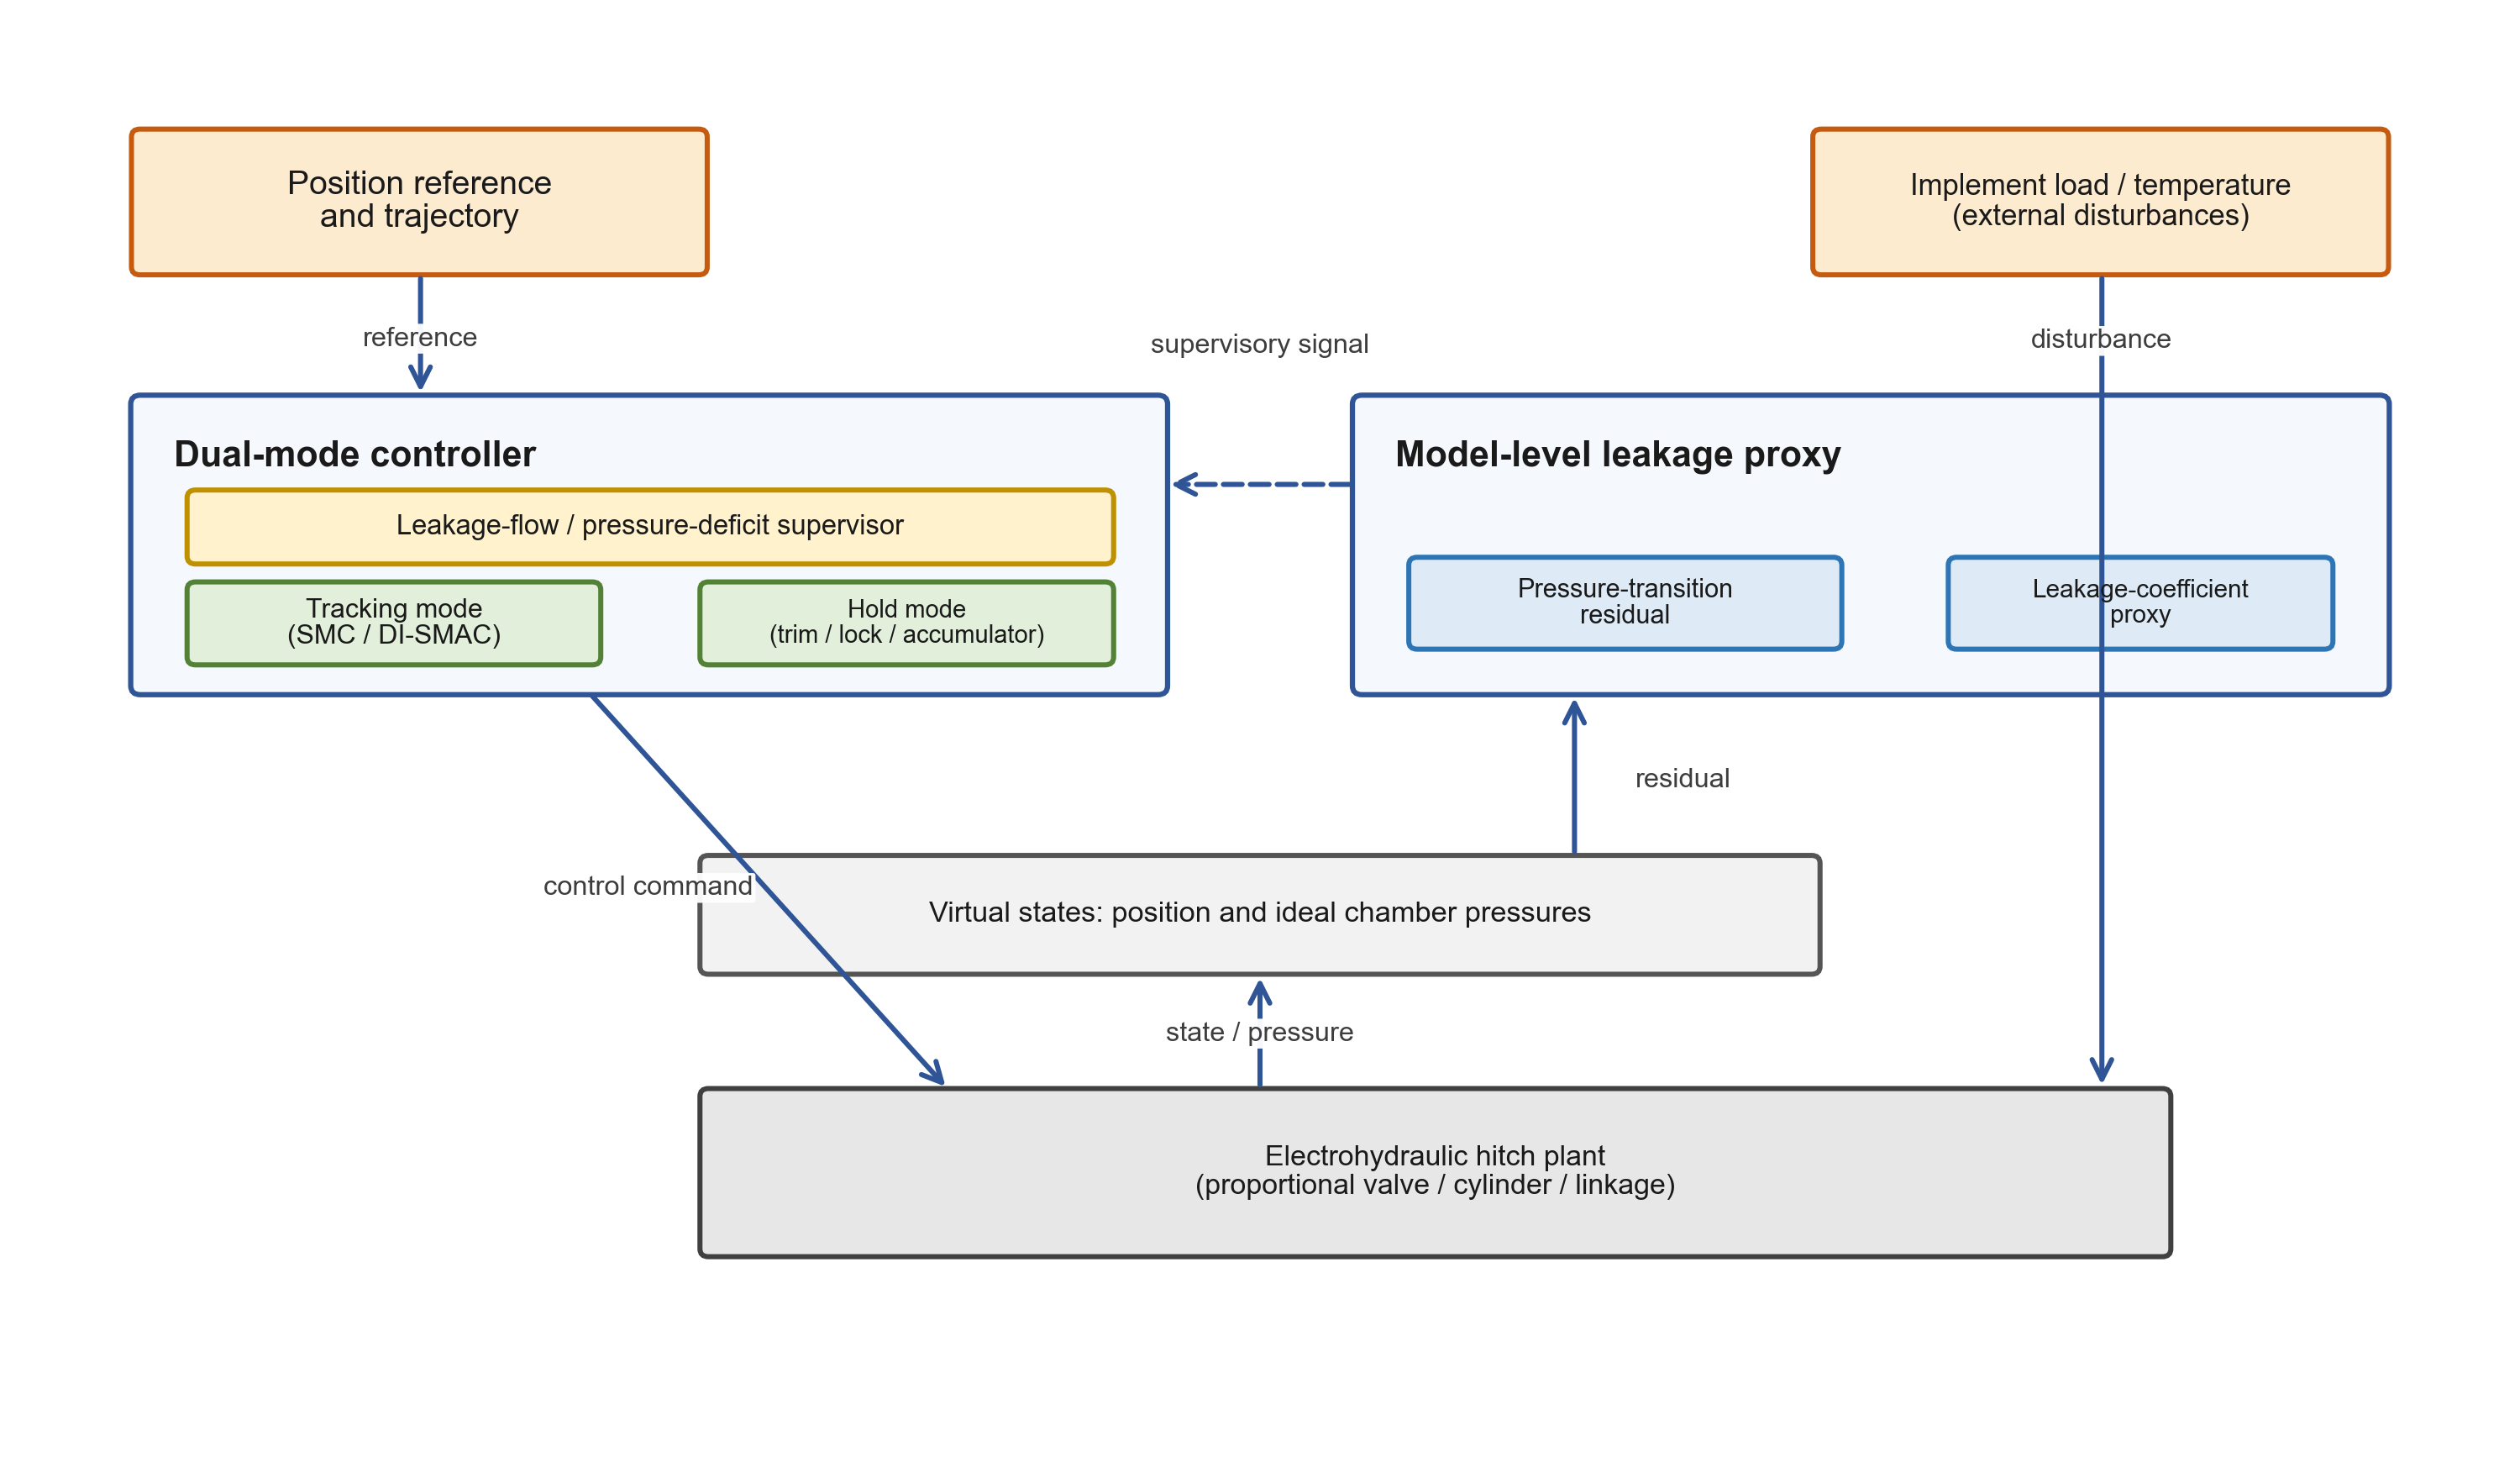
\includegraphics[width=0.96\linewidth]{paper1_architecture.png}
\caption{Dual-mode hitch-control architecture with a model-level pressure-transition leakage proxy.}
\label{fig:architecture}
\end{figure}

\subsection{Boundedness argument}
The analysis assumes bounded load and leakage-rate variation, bounded inversion error, a bounded valve command, and operation below the relief-pressure limit. For a bounded candidate error $\epsilon_k=C^*_{l,k}-C_l$, the observation error $\tilde C_l=C_l-\hat C_l$ obeys
\begin{equation}
|\tilde C_{l,k+1}|\le(1-\alpha)|\tilde C_{l,k}|+\alpha\bar\epsilon.
\end{equation}
Thus, for $0<\alpha<1$, the proxy is ultimately bounded by the virtual-model inversion error. This statement does not survive unmodelled pressure-sensor, valve, or accumulator errors without further analysis. For the sliding variable $s=\lambda(x_r-x)+v$, the boundary-layer controller gives a negative drift outside the boundary layer when the switching gain exceeds the disturbance and noise bounds. Finally, if residual hold leakage is bounded by $\bar q_l$, a conservative screening condition is
\begin{equation}
\Delta x_{1800}\le \frac{1800\bar q_l}{A}+\Delta x_{valve}+\Delta x_{structure}.
\label{eq:drop}
\end{equation}
Equation~\eqref{eq:drop} is a parameterized criterion, not proof of a physical-hardware requirement.

\subsection{Simulation protocol and statistics}
The virtual prototype was simulated at 10 ms for 1800 s. Position followed a smooth 0.15 m to 0.35 m reference over 8 s. The load was 9 kN for the first 10 s and 7 kN afterwards; oil temperature rose from 25 to 40 $^\circ$C; position-noise standard deviation was 1.5 mm. Twenty seeds (2026--2045) were used for the primary, temperature-load, and leakage-step protocols. The one-at-a-time range screen used five fixed seeds (2026--2030), because it is a deterministic assumption check rather than a field-trial estimator. The complete hybrid controller was compared with anti-windup PID, DI-SMAC, and boundary-layer SMC; all methods used the same plant, reference, noise sequence, and common hold supervisor.

The outcome metrics were full-run RMSE, terminal position error, hold-entry time, 1800 s position drop, command energy, and hold-entry rate. The filtered velocity gate, raw velocity gate, and their conjunction were evaluated separately. Ablations removed load feedforward, accumulator closed-loop compensation, the leakage proxy, hysteresis, or the hold structure. A 14 kN step, leakage multipliers, and a 60 s cylinder-leakage step from one to eight times nominal were used as virtual stress tests.

\section{Results}
\subsection{Nominal tracking and holding}
Table~\ref{tab:main} gives the 20-seed results under the filtered-velocity definition. The controllers have similar RMSE because they share the pressure feedforward and hold supervisor. The approximately 200 mm dynamic maximum error is the initial 0.20 m commanded displacement and must not be interpreted as steady-state tracking error. The hybrid controller had 4.27 mm terminal error and 0.022 mm mean hold drop.

\begin{table}[H]
\centering
\caption{Results for the parameterized 1800 s test (mean $\pm$ standard deviation, $n=20$). Hold-entry rate uses the filtered velocity gate.}
\label{tab:main}
\resizebox{\textwidth}{!}{%
\begin{tabular}{lrrrrr}
\toprule
Controller & RMSE (mm) & Terminal error (mm) & Hold entry (s) & Hold drop (mm) & Entry rate \\
\midrule
PID & $9.179\pm0.004$ & $4.138\pm0.253$ & $8.207\pm0.116$ & $0.017\pm0.021$ & 100\% \\
DI-SMAC & $9.233\pm0.008$ & $4.288\pm0.277$ & $8.464\pm0.190$ & $0.019\pm0.023$ & 100\% \\
Boundary-layer SMC & $9.228\pm0.005$ & $4.254\pm0.266$ & $8.503\pm0.181$ & $0.014\pm0.020$ & 100\% \\
Dual-mode hybrid & $9.236\pm0.006$ & $4.267\pm0.296$ & $8.523\pm0.157$ & $0.022\pm0.027$ & 100\% \\
\bottomrule
\end{tabular}
}
\end{table}

The raw-velocity and dual-gate definitions produced zero hold entries in all 20 runs. This is a material result: filter delay is part of the present hold-entry behavior, so the filtered result cannot be treated as a direct safety statement for a real hitch.

\subsection{Leakage and load-step stress tests}
Figure~\ref{fig:leak} shows the lock-valve leakage-path sensitivity. The mean drop remained below 0.088 mm at ten times the assumed lock-path leakage. This margin only describes the low-leakage parameterization. It cannot replace temperature-dependent lock-valve measurements.

\begin{figure}[H]
\centering
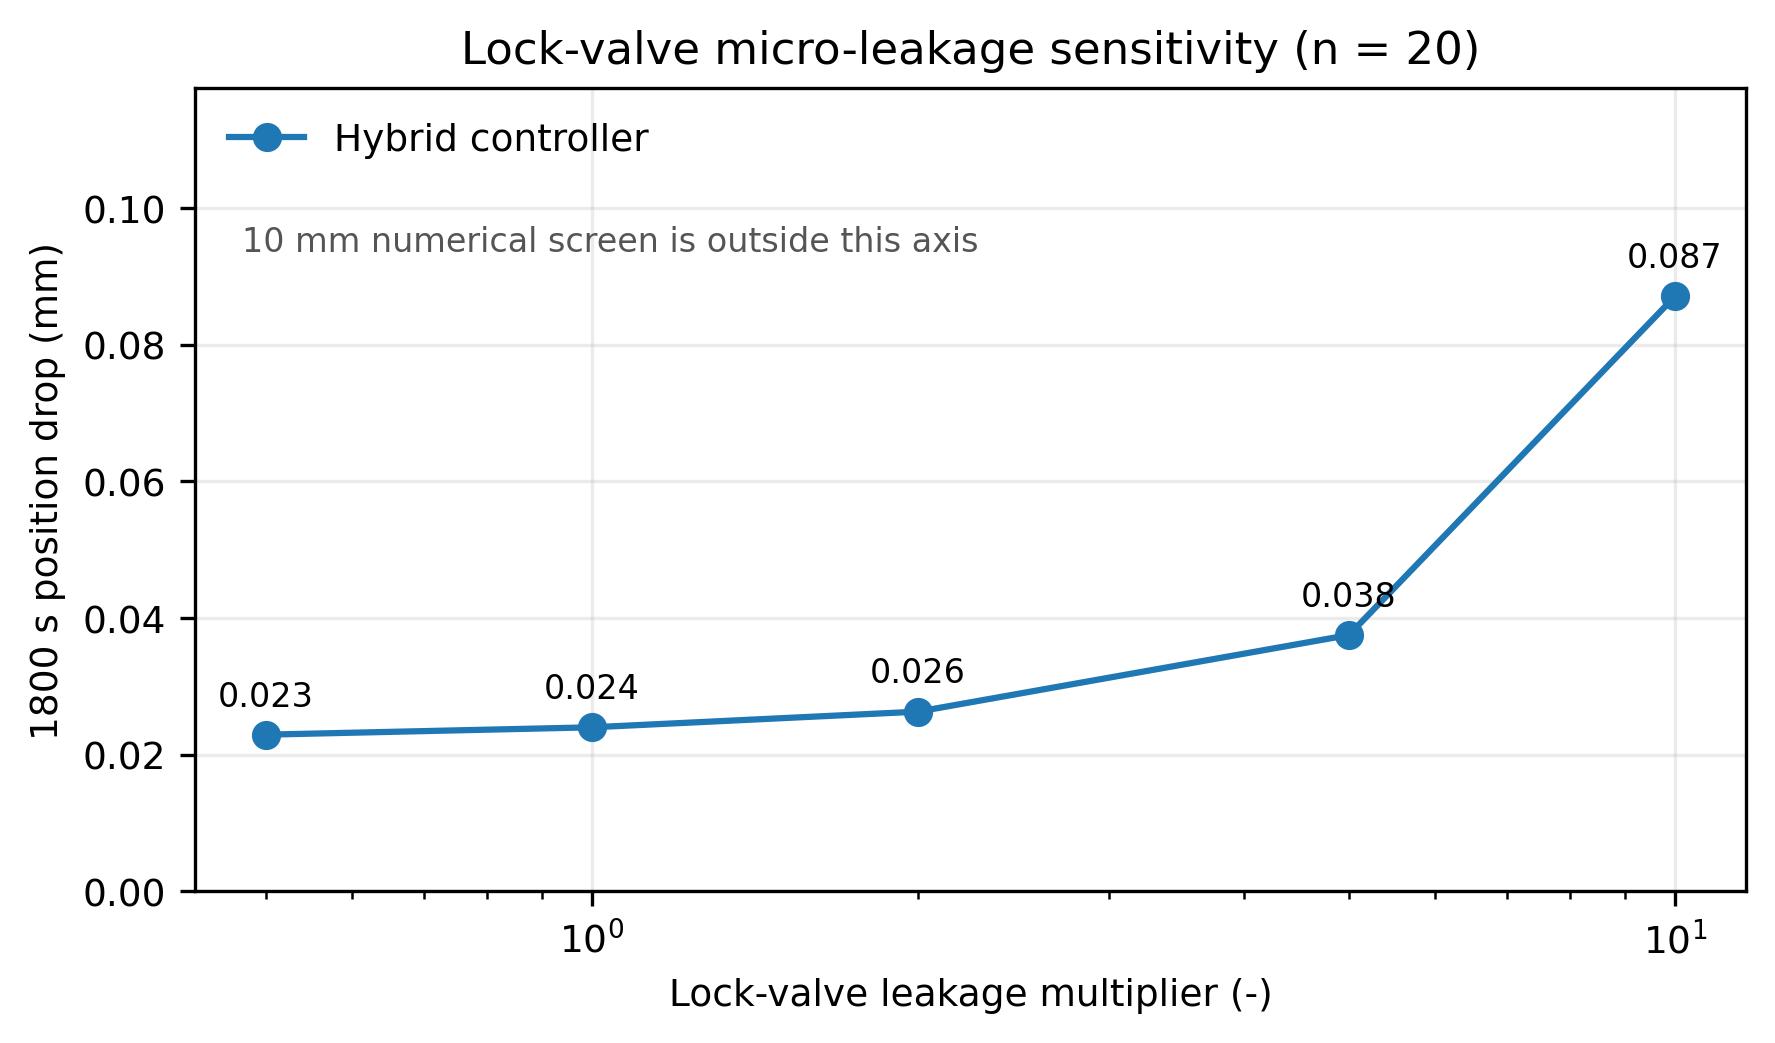
\includegraphics[width=0.76\linewidth]{paper1_lock_leakage_sensitivity.png}
\caption{Sensitivity of the complete controller to the assumed lock-valve micro-leakage path ($n=20$).}
\label{fig:leak}
\end{figure}

The more discriminating ablation is the 14 kN load step (Figure~\ref{fig:ablation}). With load feedforward and accumulator closed-loop compensation, the mean drop was 1.75 mm. Removing the accumulator closed loop increased it to 20.85 mm, and removing load feedforward increased it to 96.59 mm. The results show that the claimed benefit is conditional on a correct load signal, the modeled pressure-deficit trigger, and available accumulator pressure.

\begin{figure}[H]
\centering
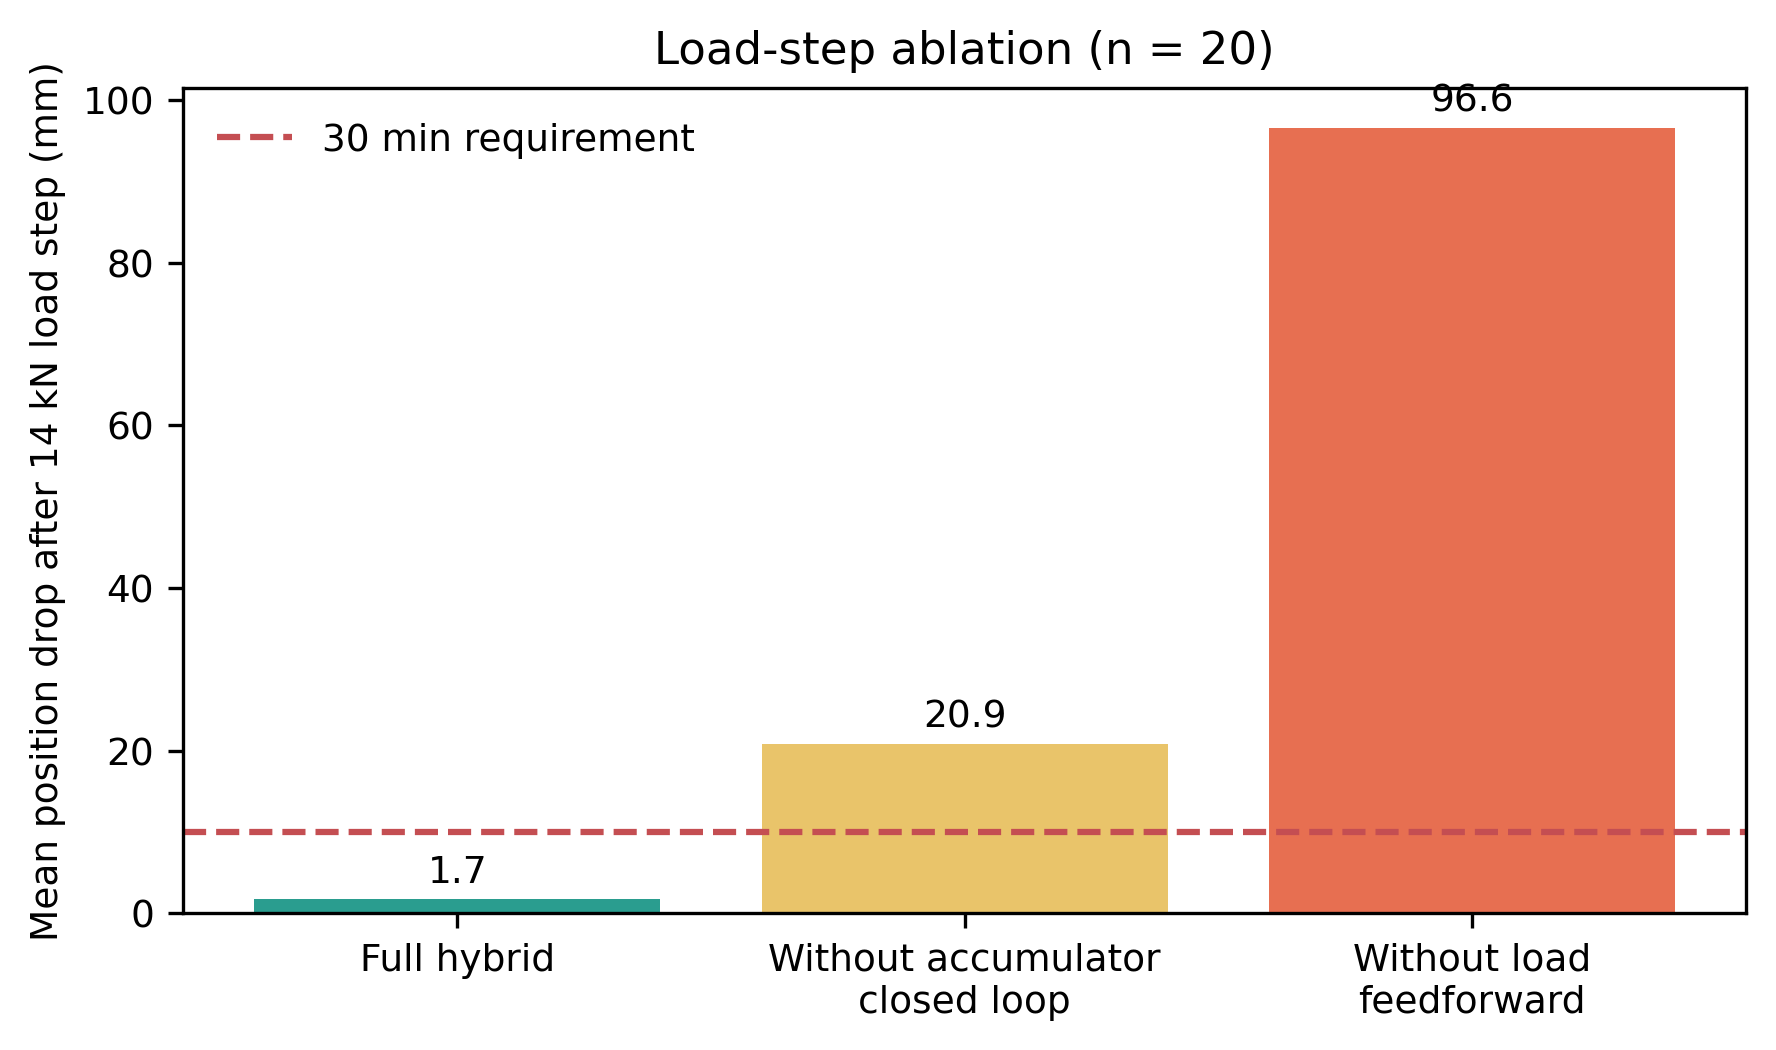
\includegraphics[width=0.76\linewidth]{paper1_load_step_ablation.png}
\caption{Load-step ablation for a 14 kN step. The dashed line is the assumed 10 mm, 30 min requirement ($n=20$).}
\label{fig:ablation}
\end{figure}

\subsection{Assumption-range and virtual leakage-step screens}
Figure~\ref{fig:assumption-proxy} summarizes selected one-at-a-time stress settings. Across the mass, damping, stiffness, position-noise, and cylinder-leakage settings in Table~\ref{tab:assumptions}, all five-seed cases entered hold and their mean 1800 s drop was below 0.060 mm. At the 14 kN step, the assumed accumulator-flow coefficient was consequential: 0.5$\times$ and 1.5$\times$ its nominal value gave mean drops of 5.86 mm and 0.273 mm, respectively. These are model-structure sensitivities, not confidence bounds on a real hydraulic circuit.

For a virtual cylinder-leakage step at 60 s from one to eight times the nominal coefficient, the pressure-transition proxy reached 90\% of the new coefficient in $0.255\pm0.005$ s ($n=20$) and ended at $1.200\times10^{-11}$ m$^3$ s$^{-1}$ Pa$^{-1}$; a fixed nominal prior remained at $1.5\times10^{-12}$ m$^3$ s$^{-1}$ Pa$^{-1}$. Both cases entered hold in 20/20 runs and had the same 0.022 mm mean drop. Thus, the test demonstrates internal state-transition and supervisory-mode consistency, not an independent position-holding advantage or physical leakage identification.

\begin{figure}[H]
\centering
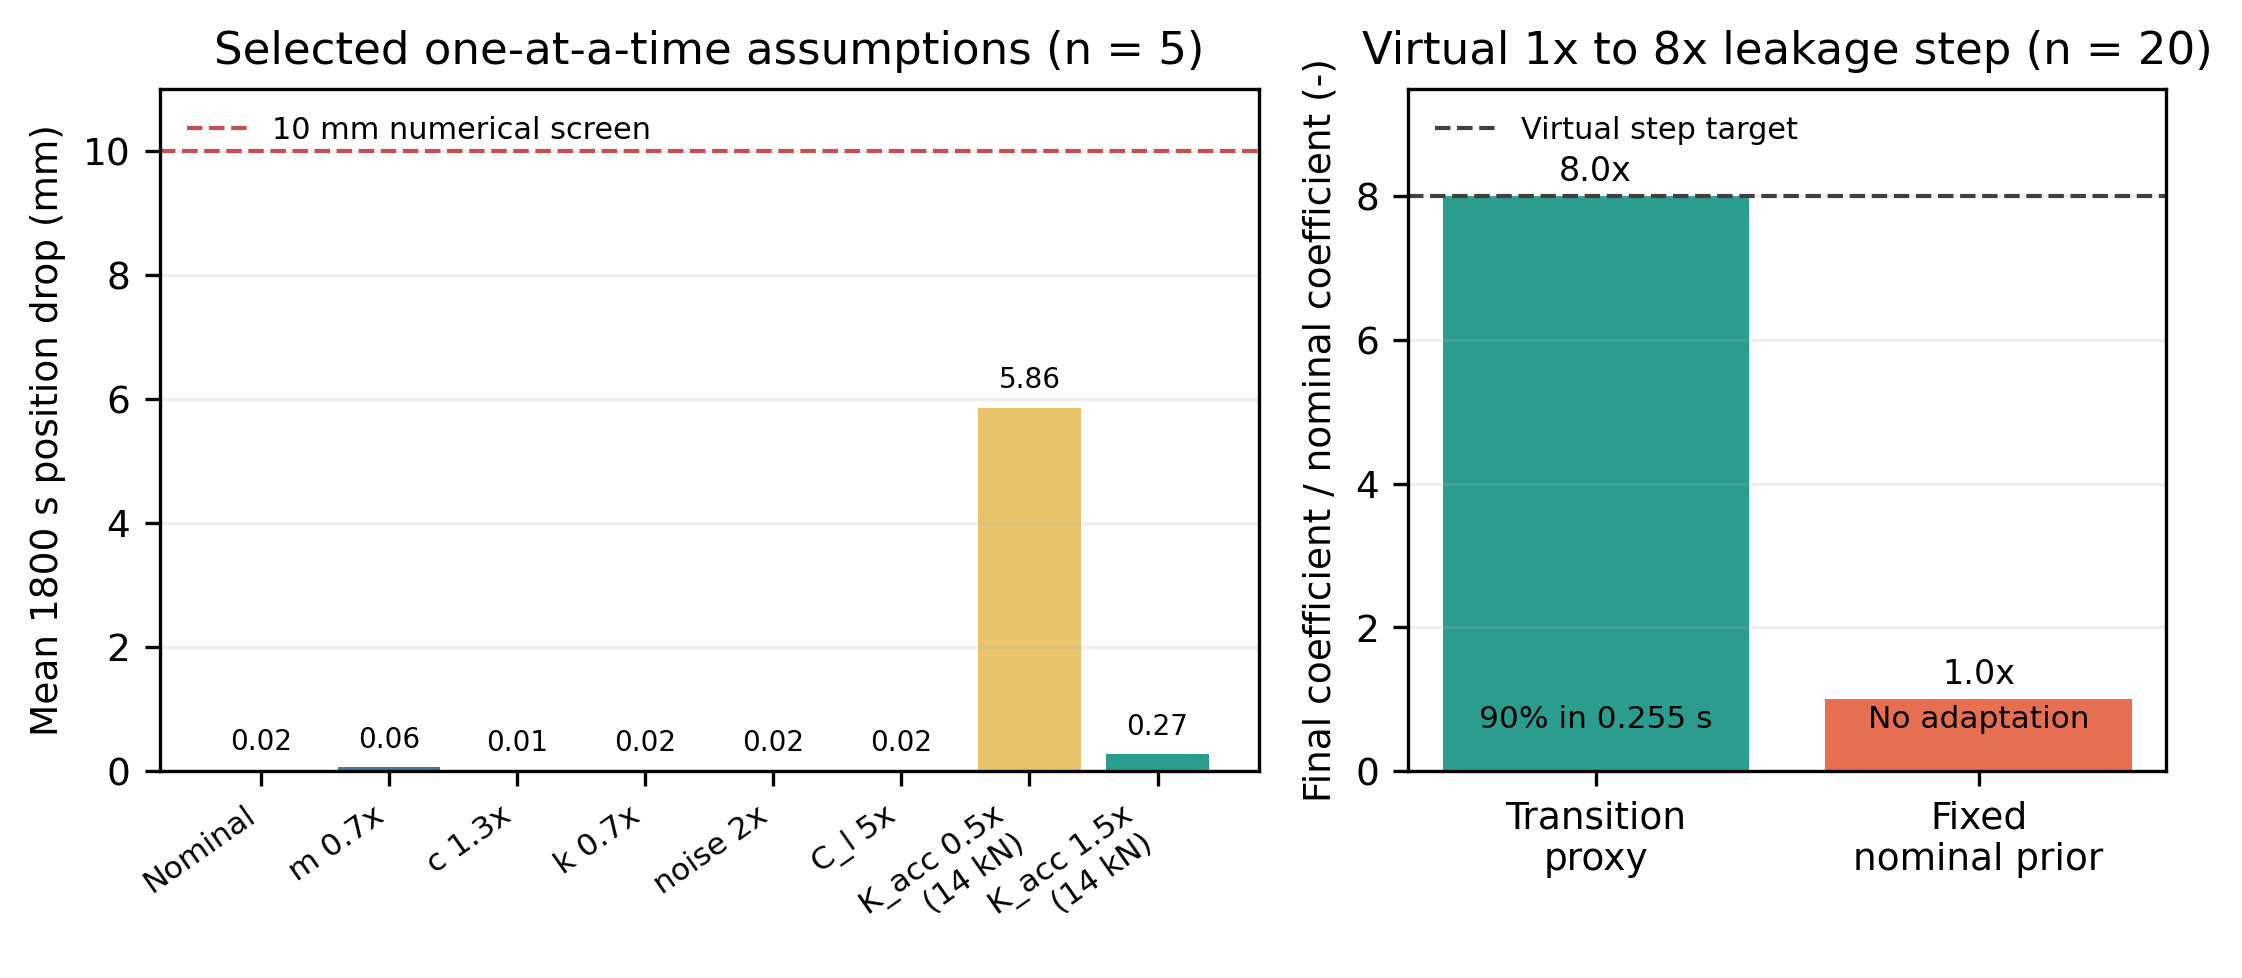
\includegraphics[width=0.94\linewidth]{paper1_assumption_and_proxy_stress.png}
\caption{Selected assumption-range screen (left, $n=5$) and virtual one-to-eight-times leakage step (right, $n=20$). Both panels are parameterized model tests, not calibrated-hitch evidence.}
\label{fig:assumption-proxy}
\end{figure}

\subsection{Temperature-load envelope and raw-velocity threshold}
The controller was next evaluated over a parameterized temperature-load envelope: constant oil temperatures of 25, 40, and 50 $^\circ$C were crossed with post-step loads of 7, 10, and 14 kN ($n=20$ per case). The filtered 3 mm s$^{-1}$ velocity gate entered hold in all nine cases. Figure~\ref{fig:envelope} shows that the highest mean 1800 s position drop was 1.93 mm (95\% CI: 1.74--2.11 mm) at 50 $^\circ$C and 14 kN. The temperature-load result broadens the virtual operating envelope, but it does not provide a physical temperature or load validation because the leakage and thermal parameters are still assumed.

The same protocol was also evaluated with an unfiltered velocity signal. At raw thresholds of 3 and 5 mm s$^{-1}$, none of the 20 runs entered hold. Relaxing the raw threshold to 10 mm s$^{-1}$ produced 20/20 entries and a 0.031 mm mean drop (95\% CI: 0.016--0.047 mm). This sensitivity result identifies a candidate signal-processing design trade-off; it does not validate the original 3 mm s$^{-1}$ requirement or establish an acceptable hardware safety threshold.

\begin{figure}[H]
\centering
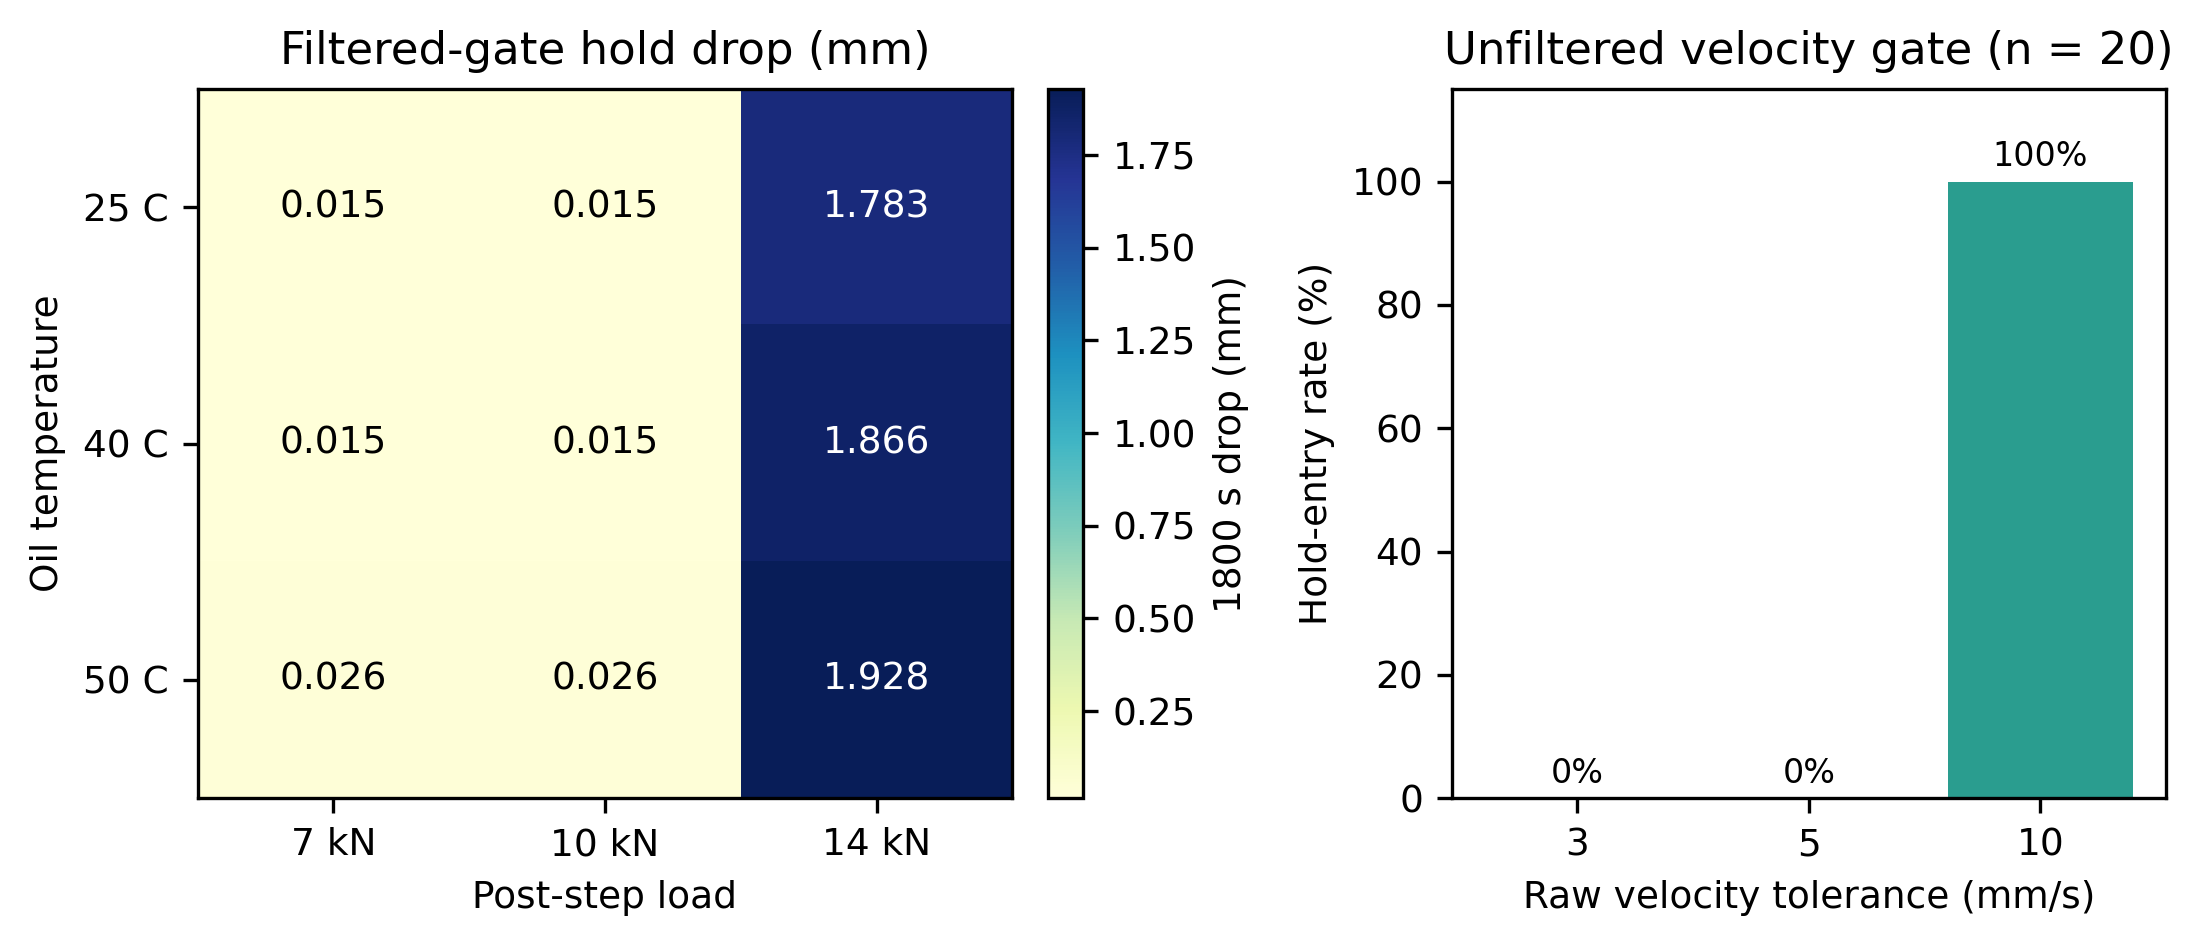
\includegraphics[width=0.94\linewidth]{paper1_operating_envelope.png}
\caption{Parameterized temperature-load envelope under the filtered velocity gate (left), and sensitivity of the unfiltered velocity gate to its tolerance (right), $n=20$ per condition.}
\label{fig:envelope}
\end{figure}

\section{Discussion}
The simulation does not support a claim that the hybrid law has intrinsically better nominal tracking than PID or DI-SMAC. Its differentiated value is an explicit holding architecture and its behavior in the load-step and temperature-load tests. The 14 kN ablation supports the modeled load-feedforward and accumulator branches. By contrast, the fixed-prior and leakage-proxy runs had identical hold drops in the leakage-step screen. The proxy should therefore be interpreted as a transparent model-state and supervisory-mode diagnostic, not as evidence of a general observer-performance benefit.

The central threats to validity are the assumed leakage paths, accumulator properties, friction, load measurement, and ideal pressure-state access. Furthermore, the 20 repetitions only perturb position-sensor noise; they are not independent field trials. The pressure-transition proxy is deliberately evaluated against the same virtual model that produces its state transition, so its rapid response is an internal-consistency result rather than validation of real leakage identification. The raw-velocity hold gate must be validated with measured sensor bandwidth before the method can be described as an implementable safety solution. The 10 mm s$^{-1}$ raw-gate result is a relaxed simulation setting, not a replacement acceptance criterion.

\section{Conclusions}
This study presents a reproducible dual-mode hitch-control virtual prototype that combines pressure feedforward, a model-level leakage proxy, a hysteretic hold supervisor, accumulator compensation, and load feedforward. Under the declared parameterization, the complete controller meets the numerical position-holding screen, attenuates a 14 kN load-step disturbance, and remains within 1.93 mm mean drop in the tested 25--50 $^\circ$C and 7--14 kN envelope. The one-at-a-time stress screen makes the dependence on assumed accumulator capacity explicit. The original strict raw-velocity gate, however, never entered hold; only a relaxed 10 mm s$^{-1}$ raw threshold entered all virtual runs. The valid contribution is a parameterized theoretical method and reproducible stress-test workflow, not a claim of physical hitch performance. Bench or vehicle experiments, identified hydraulic parameters, and measured pressure/velocity sensing are future work required only for physical-performance or deployment claims.

\authorcontributions{Conceptualization, C.C.; Methodology, C.C.; Software, C.C.; Formal analysis, C.C.; Visualization, C.C.; Writing---original draft preparation, C.C.; Resources, C.C.; Validation, Z.Z.; Investigation, L.W.; Writing---review and editing, Z.L. and Y.Z.; Supervision, Z.L. and Y.Z.; Project administration, Y.Z.; Funding acquisition, Y.Z.}
\funding{This work has received funding from the Science and Technology Project of the Ministry of Agriculture and Rural Affairs of China.}
\institutionalreview{Not applicable.}
\informedconsent{Not applicable.}
\dataavailability{The virtual-prototype source code, reproduction scripts, machine-readable parameter manifest, assumption register, traceability exporter, and JSON outputs supporting these results are publicly available at \url{https://github.com/Fat-pig-Cui/agricultural-tractor-virtual-prototypes}. The Zenodo version DOI for the archival release will be added before publication.}
\acknowledgments{During preparation of this manuscript, the authors used OpenAI Codex for English translation, language editing, and development of plotting scripts. The authors must review and edit all output and take full responsibility for the content before submission.}
\conflictsofinterest{The authors declare no conflicts of interest.}

\begin{thebibliography}{9}
\bibitem{bai2010} Bai, Y.; Li, P. Adaptive fuzzy sliding mode control for electro-hydraulic position servo system. \emph{2010 Chinese Control and Decision Conference} 2010, 3249--3253. \url{https://doi.org/10.1109/CCDC.2010.5498613}.
\bibitem{tang2011} Tang, R.; Zhang, Q. Dynamic sliding mode control scheme for electro-hydraulic position servo system. \emph{Procedia Engineering} \textbf{2011}, \emph{24}, 28--32. \url{https://doi.org/10.1016/j.proeng.2011.11.2596}.
\bibitem{jin2013} Jin, B. Chattering inhibition of variable rate reaching law sliding mode control for electro-hydraulic position servo system. \emph{Journal of Mechanical Engineering} \textbf{2013}, \emph{49}, 163--169. \url{https://doi.org/10.3901/JME.2013.10.163}.
\bibitem{kim2025} Kim, E.-K.; Han, T.-H.; Lee, J.-H.; Han, C.-W.; Lim, R.-G. Tracking accuracy evaluation of autonomous agricultural tractors via rear three-point hitch estimation using a hybrid model of EKF-Transformer. \emph{Agriculture} \textbf{2025}, \emph{15}, 1475. \url{https://doi.org/10.3390/agriculture15141475}.
\bibitem{liu2023} Liu, C.; Gu, J.; Du, X.; Liu, C.; Du, Y.; Mao, E. Differential and integral sliding mode adaptive control algorithm for draft and position integrated control of electro-hydraulic hitch in agricultural tractor. \emph{INMATEH Agricultural Engineering} \textbf{2023}, \emph{70}, 369--378. \url{https://doi.org/10.35633/inmateh-70-36}.
\end{thebibliography}
\end{document}
